
\section*{Kondensatoren}

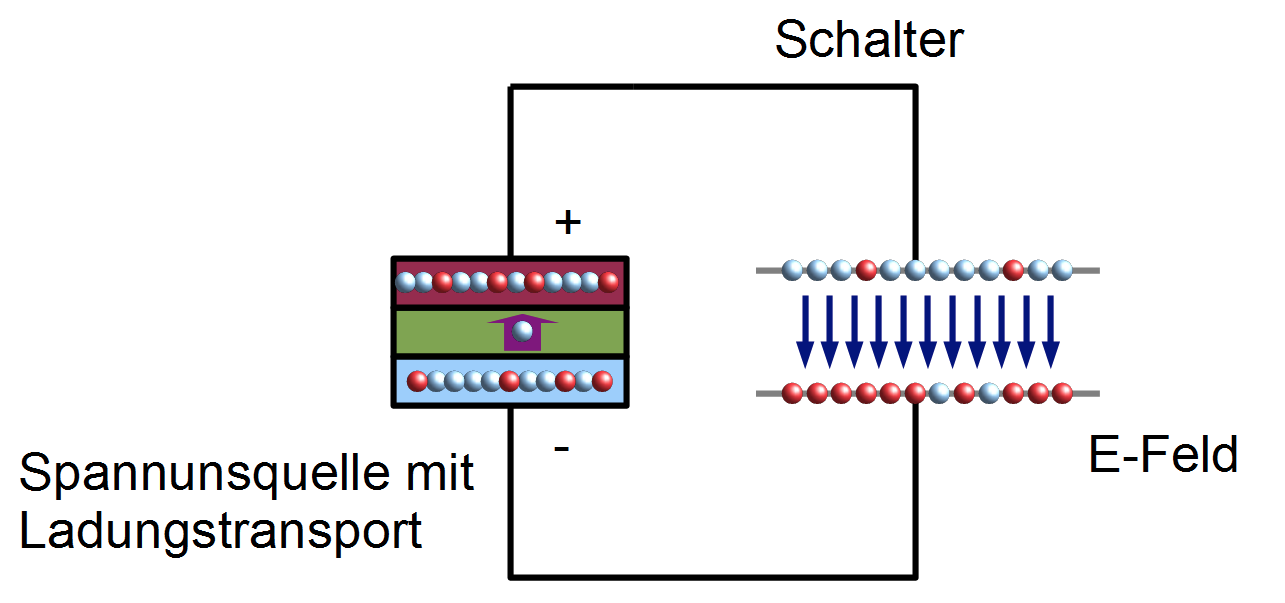
\includegraphics[width=6cm]{El-Felder-Stroeme/kondensator1}

\begin{tabular}{|l|l|c|}
\hline 
Spannung & $U=-\int_{Unterseite-Kondensator}^{Oberseite-Kondensator}\vec{E}d\vec{r}=\frac{QL}{A\varepsilon_{0}}$ & \multirow{3}{*}{%
\begin{tabular}{|l|}
\hline 
Q= Ladung\tabularnewline
\hline 
L= Distanz der Platten\tabularnewline
\hline 
\end{tabular}}\tabularnewline
\cline{1-2} 
 &  & \tabularnewline
\cline{1-2} 
 &  & \tabularnewline
\hline 
\end{tabular}$ $
